\section{A szimuláció eredményei}
\begin{frame}
	\frametitle{A szimuláció eredményei}
	\begin{block}{Adatok összevetése}
		A már rendelkezésünkre álló bemeneti paraméterekre\cite{archetti2016cooperation} elvégeztünk 100-100 szimulációt, minden egyes diffúziós távolságra 1-től 5-ig.
	\end{block}

	\begin{block}{Paraméterek}
		\begin{multicols}{2}
			\begin{itemize}
				\item populáció mérete: 1000
				\item defektálók: 5\%
				\item generációk száma: 15
				\item kooperálók költsége: 0.01
				\item osztódás: nincs
			\end{itemize}
			\begin{itemize}
				\item $s = 20$
				\item $k = 0.5$
				\item $d = \frac{1}{2}D$
				\item $z = 3$
			\end{itemize}	
		\end{multicols}
	\end{block}
\end{frame}

\begin{frame}
	\frametitle{Összehasonlítás}
	\begin{figure}[h]
		\centering
		\begin{tabular}{cc}
			\includegraphics[width=0.4\linewidth]{images/dist4}
			&
			\includegraphics[width=0.4\linewidth]{images/dist5}
			\\
			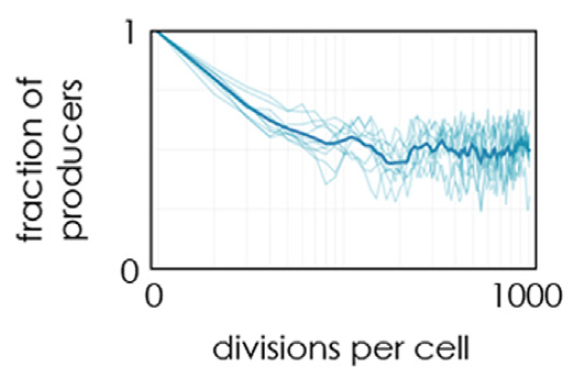
\includegraphics[width=0.4\linewidth]{images/arc_dist4}
			&
			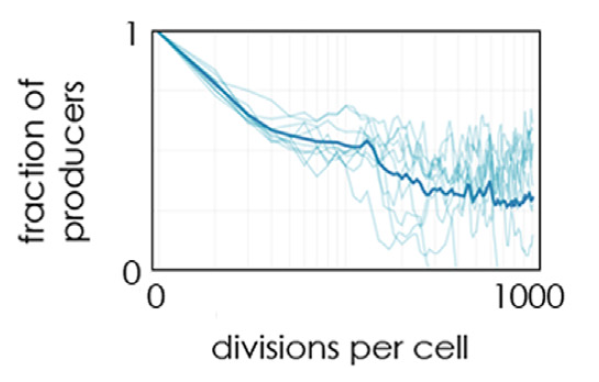
\includegraphics[width=0.4\linewidth]{images/arc_dist5}
			\\
		\end{tabular}
		\caption{Szimulációs eredmények a fenti paraméterekre és azok párjai a \cite{archetti2016cooperation} cikkből}
		\label{fig:DistChange}
	\end{figure}
\end{frame}

\subsection{A költség és nyereség hatása}
\begin{frame}
	\frametitle{A költség és nyereség hatása}
	\begin{block}{}
			\begin{itemize}
				\item sokba kerül a termelés $\Rightarrow$ megéri élősködni
				\item alacsony költség $\Rightarrow$ fenntartható egy bizonyos egyensúly
			\end{itemize}
	\end{block}

	\begin{figure}[h]
		\centering
		\begin{tabular}{cc}
			\includegraphics[width=0.35\linewidth]{images/chart001.jpeg}
			&
			\includegraphics[width=0.35\linewidth]{images/chart01.jpeg}
		\end{tabular}
		\begin{tabular}{cl}  
			\begin{tabular}{c}
				\includegraphics[width=0.35\linewidth]{images/chart08.jpeg}
			\end{tabular}
			& 
			\begin{tabular}{l}
				\parbox{0.35\linewidth}{
					A játék végkimenetele mikor a költségek rendre 0.01, 0.1 és 0.8
				}
			\end{tabular}  \\
		\end{tabular}
		\label{fig:CoopCostChange}
	\end{figure}
\end{frame}

\subsection{Diffúziós távolság hatása}
\begin{frame}
	\frametitle{Diffúziós távolság hatása}
	\begin{itemize}
		\item a diffúziós távolság növelésével valósághűbb adatokat kaphatunk
		\item a távolság növekedésével a defektáló sejtek könnyebben terjednek
		\item ezt a paramétert a hasnyálmirigyrák esetén megállapították\cite{archetti2015heterogeneity}
	\item az esetek túlnyomó részében ez az érték 5-10-től 30-60-ig terjedhet\cite{archetti2016cooperation}
	\end{itemize}
	
	\begin{figure}[h]
		\centering
		\begin{tabular}{cc}
			\includegraphics[width=0.4\linewidth]{images/diffdist2}
			&
			\includegraphics[width=0.4\linewidth]{images/diffdist5}
		\end{tabular}
		\caption{A játék végkimenetele két diffúziós távolságra. A paraméterek: 160 sejt, 5\% defektáló, 0.3 költség, távolság: 2 illetve 5}
		\label{fig:DiffDist}
	\end{figure}
\end{frame}

\subsection{Osztódásra képes populációk}
\begin{frame}
	\frametitle{Osztódásra képes populációk}
	\begin{itemize}
		\item eddigi a populáció mérete állandó volt és egy adott modellt követett
		\item a valóságban a defektáló sejtek nem csak területileg terjednek el
		\item számosságban is túlnövik a kooperálókat
	\end{itemize}
	
	\begin{columns}
		\column{0.5\textwidth}
			\begin{figure}[ht]
				\centering
				\begin{tabular}{c}
					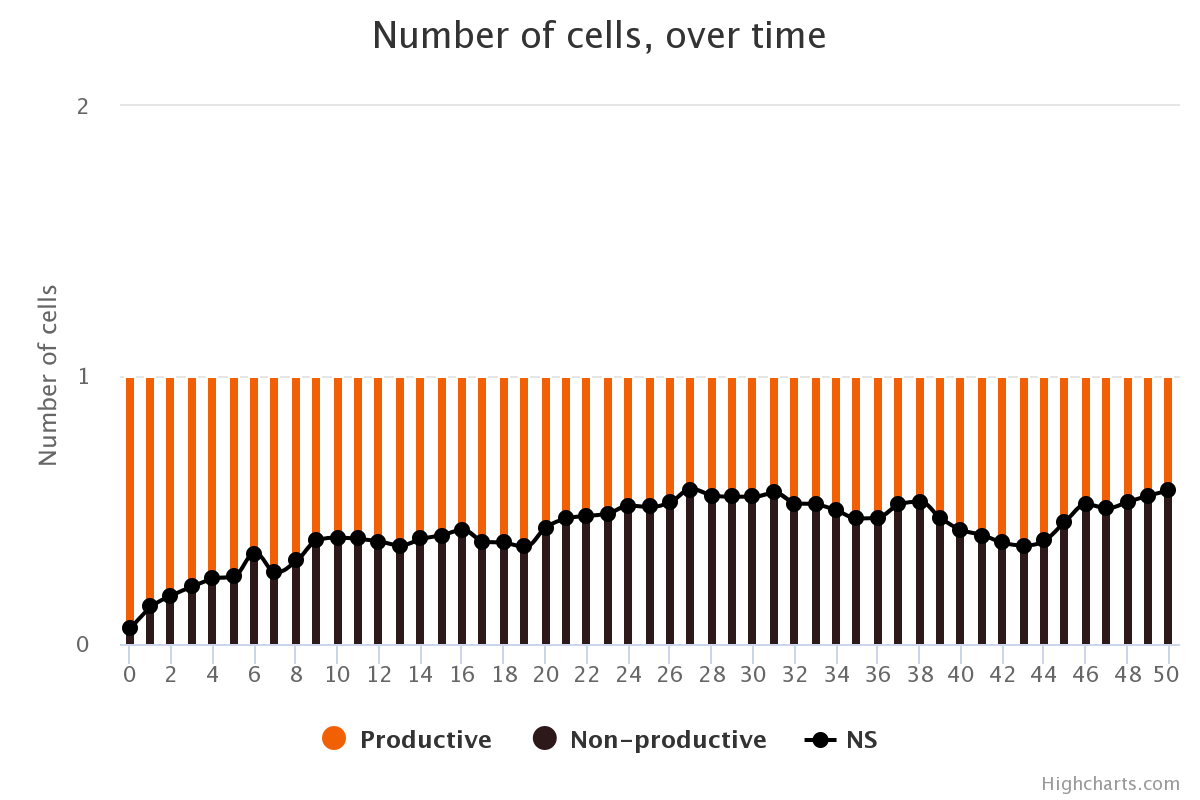
\includegraphics[width=0.9\textwidth]{images/nemosztodik}
					\\
					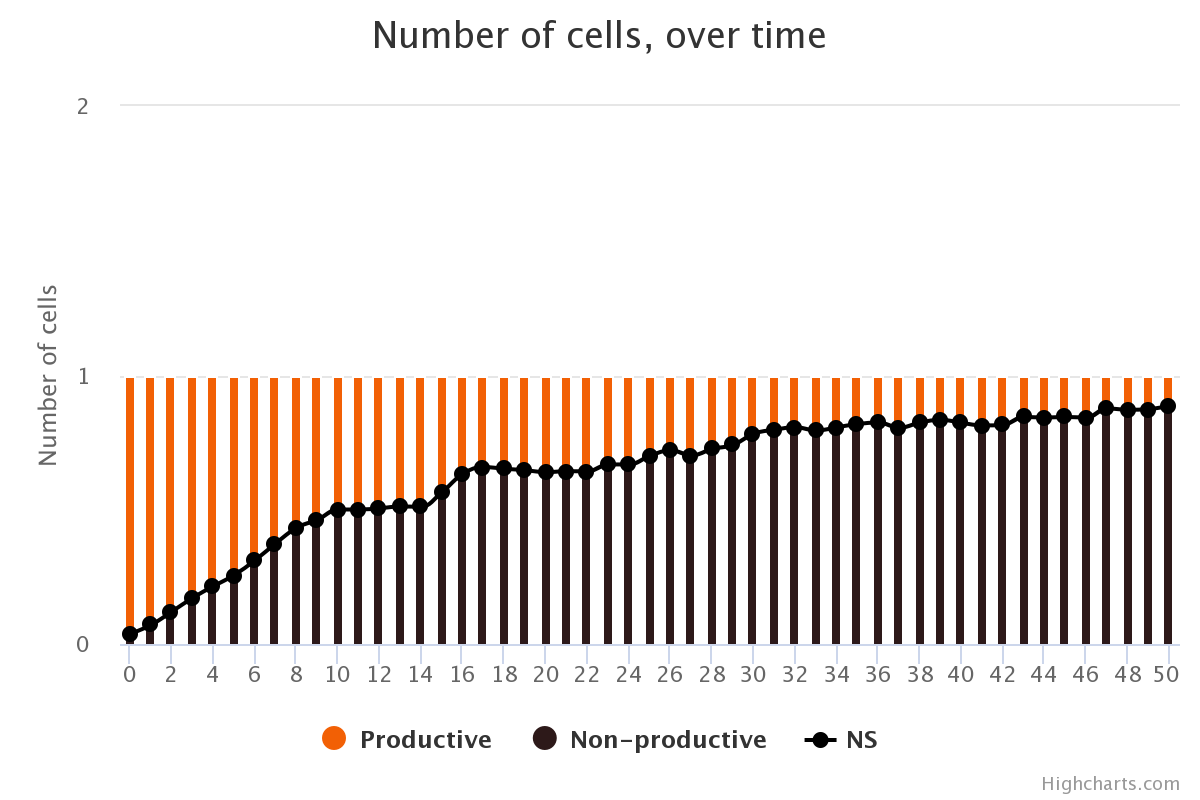
\includegraphics[width=0.9\textwidth]{images/osztodik}
				\end{tabular}
				\caption{Az első esetben a sejtek nem osztódtak míg a másodikban igen}				
				\label{fig:Divide}
			\end{figure}
		\column{0.5\textwidth}
			\begin{block}{}
				\begin{itemize}
					\item az új sejtek képesek felgyorsítani a defektálók terjedését
					\item további kísérletek szükségesek
				\end{itemize}
			\end{block}
	\end{columns}
\end{frame}

\begin{frame}
	\frametitle{Osztódással vagy anélkül?}
	\begin{figure}
		\centering
		\includegraphics[width=\linewidth]{images/oszotas_nemosztodas}
		\caption{Osztódást nem használó és használó modell}
	\end{figure}
\end{frame}
